\documentclass{school-22.211-notes}
\date{May 23, 2012}

\begin{document}
\maketitle

%%%%%%%%%%%%%%%%%%%%%%%%% Qualify Exam Start %%%%%%%%%%%%%%%%%%%%%%%%%%%%
\lecture{Qualify Exam Recap}
%Kord mentioned 09/10/12 that Prompt jump approximation is a classical qual problem.

\topic{Basics (with questions)}
\begin{enumerate}
\item Common units, see Table~\ref{units}. Angular flux is scalar quantity and the term with angular dependency is $n$ not $v$. 
\begin{table}[ht]
  \centering
  \begin{tabular}{|c|c|c|c|c|c|} \hline
   $\sigma$ & $\Sigma$ & $\phi = nv$  & $J$ & $R = \phi \Sigma$ & RI  \\ \hline
   $\cm^2$ & $1/\cm$ & $\frac{n}{\cm^2 \s}$  & $\hat{e} \frac{n}{\cm^2 \s}$ & $\frac{\mathrm{reactions}}{\cm^3 \s}$ & barns \\ \hline
  \end{tabular}
  \caption{Units of Common Terms} \label{units}
\end{table}
\item 1 GWd/MT = 30 days = 30 million dollars. 
\item Boron worth: -16 pcm/ppm. Approximate as -10 pcm/ppm. 
\item PWRs have 20\% $\Delta k$ reactivity hold-down, whereas BWRs only have 2\% (b/c the use of Gd; Gd behaves like onion skin burning; Gd can control burning by density). 
\item Fast flux in hydrogen is around $10^{14}$ n/cm$^2$s, and on the order of $10^{12}$n/cm$^2$s for thermal flux. 
\item Average energies prompt neutrons are released: 2 MeV (peak prompt neutron energies: 0.7 MeV). Average energies delayed neutrons are released: 0.4 MeV. 
\item Core decay heat after 1 day is about 1\% rated. 
\item Constants to know: 1u = 931.5 MeV. 
\item The effect of U238 energy self-shielding is about an effect of 10, that is, going from infinite dilution to U/I = 0.1. 

\item Reactivity units. 
\begin{table}[ht]
  \centering
  \begin{tabular}{|c|c|c|} \hline
    Unit & Definition & Example \\ \hline
    $\Delta k$ & actual units of PKEs & 0.01 \\
    \% $\Delta k$ & & 1\% \\
    pcm & $10^5 \Delta k $ & 1000 pcm \\ \hline
    Dollars & $\frac{\Delta k}{\beta}$ & \$1.5 \\
    Cents & 100 Dollars & 150 cents \\ 
    Milli-beta & 1000 Dollars & 1500 milli-beta \\ \hline
  \end{tabular}
\end{table}
\end{enumerate}

\clearpage
\textbf{General Knowledge Practice Questions}
\begin{enumerate}
\item (Qual 2012). 
\begin{enumerate}
\begin{figure}[ht]
  \centering
  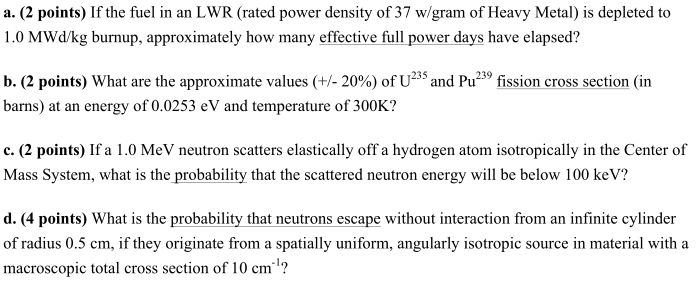
\includegraphics[width=6in]{images/qual/general_knowledge.png}
\end{figure}
\item We approximate 1 GWd/MT (that is 1 MWd/kg) as 30 days of operation. 

\item Fission cross section at 0.1eV and 300K for \ce{U^{235}} is 250b, for \ce{Pu^{239}} is about 475b. 

\item The pdf is a flat distribution, so it is equally likely to get anywhere below 1.0 MeV, then the change of below 100 keV is 100 keV/1 MeV = 10\%. 

\item We treat this as a fuel to moderator two-region problem. Then we can calculate fuel to fuel probability. First we calculate chord length $l = \frac{4V}{S} = \frac{4 \pi r^2 H}{2 \pi r H} = 2r = 1\fsp \cm.$
\eqn{ P_{FF} = \frac{\Sigma_t^F (u)}{\Sigma_t^F (u) + \Sigma_e}  = \frac{10}{10 + 1} = 0.909 } 
Thus the probability of escaping the cylinder is just 9.09\%. 
\end{enumerate}

\item (12 Final \#1-20) 
  \begin{enumerate}
  \item What are the average energies at which prompt and delayed fission neutrons are emitted? \\
    \textbf{Answer:} 2 MeV for prompt neutrons, 0.4 MeV for delayed neutrons. 

  \item What are the units of real and adjoint flux?\\
    \textbf{Answer:} Real flux has a unit of neutrons per cm$^2$ per second. Adjoint flux is typically unitless. 

  \item What is the difference between true and `effective' downscatter in two-group cross sections? \\
    \textbf{Answer:} True down-scattering cross section $\Sigma_{s,1\to 2}$ measures the probability of scattering from group 1 to group 2. Effective down-scattering cross section $\displaystyle \hat{\Sigma}_{s,1\to 2} = \Sigma_{s,1\to 2} - \Sigma_{s, 2 \to 1} \frac{\phi_2}{\phi_1}$ is like combining flux-weighted up-scattering and down-scattering into one down-scattering term. 

  \item What phenomenon is responsible for the $1/v$ tail of thermal scattering cross sections for isotopes with constant elastic cross sections at higher energies?\\
    \textbf{Answer:} Thermal motion/thermal vibration of the interaction material. 

  \item What is the mean number of isotropic elastic scattering collisions with Livermorium, \ce{Lv_{116}^{293}}, required to slow neutrons from 1 MeV to 1.0 eV? \\
    \textbf{Answer:} $\displaystyle A = 293, \alpha = \left( \frac{A-1}{A+1} \right)^2 = 0.986, \xi = 1 + \frac{\alpha \ln \alpha}{1 - \alpha} = 6.8 \times 10^{-3}, n = \frac{\ln (E_2 / E_1)}{\xi} = 2028.6.$ Hence it requires 2029 collisions. 

  \item What is the average spacing (in eV) of \ce{U^{238}} resolved capture resonances? \\
    \textbf{Answer:} 25 eV. 

  \item For Einsteinium \ce{Es^{253}} in the energe range from 11.102 eV to 99.653 eV, what is the ratio of group absorption cross section to resonance integral? \\
    \textbf{Answer:} Recall that $\RIeff$ and $\sigma_g$ are related through: $\displaystyle \RIeff = \sigma_g \ln \left(\frac{E_2}{E_1} \right)$, hence the ratio is, $\displaystyle \frac{\sigma_g}{\RIeff} = \frac{1}{\ln  \left(\frac{E_2}{E_1} \right) } = 0.456$. 

  \item What is the definition and units of `dilution cross section' for resonance absorbers? \\
    \textbf{Answer:} Dilusion cross section is defined as, 
    \eqn{ \sigma_d = \frac{N_m r_m}{N_r} }
    where $N_m, r_m$ are the number density and cross section of the moderating material, and $N_r$ is the number density of the resonant material. $\sigma_d$ has the unit of $\cm^2$. 

  \item What is the approximate flux disadvantage factor at 0.5 eV for a 17x17 PWR lattice? \\
    \textbf{Answer:} Notice flux disadvantage factor seem to be defined two ways: 
    \begin{itemize}
    \item The moderator flux over the fuel flux (as in Reuss' book, e.g. Fig. 9.4) in which case the flux disadvantage factor would be about 1.05 for standard fuel, 1.1 for MOX fuel. 
    \item The fuel flux over the moderator flux as in Kord's lectures, in which case the flux disadvantage factor would be around 0.9
    \end{itemize}
    Hence results within 0.9 to 1.1 receive credits for this problem. 

  \item What is the approximate Doppler temperature coefficient in pcm/K in an LWR? \\
    \textbf{Answer:} -3 pcm/K (it is important that the Doppler coefficient is negative), see slide 17, Lecture 10. 

  \item What are the two primary sources for the production of \ce{Xe^{135}}? \\
    \textbf{Answer:} Iodine decay (major source), fission/burnup (minor source). 

  \item What is resonance escape probability for a material with a resonance integral of 100 barns, a dilution cross section of 2000 barns, and a mean logarithmic energy decrement of 0.333? \\
    \textbf{Answer:} Recall the expression for resonance escape probability: 
    \eqn{ p \approx \exp \left( - \frac{\RIeff}{\xi \sigma_d} \right) = \exp \left( - \frac{100 b}{0.333 \times 2000 b} \right) = 0.861 }

  \item What is Dancoff factor for unclad PWR fuel rods with radius 0.5cm in a voided uniform infinite lattice with a pitch of 1.99 cm? \\
    \textbf{Answer:} When the moderator is void, that is the opacity is zero, hence Dancoff factor is 1.0. 

  \item What is the difference between delayed neutron fraction and delayed neutron yield? \\
    \textbf{Answer:} Absolute delayed neutron yield is the number of delayed neutrons per fission. Relative delayed neutron yield is the number of delayed neutrons per fission for an isotope divided by number of delayed neutrons per fission for all isotopes. Delayed neutron fraction is the absolute yield divided by $\bar{\nu}$. 

  \item What are the approximate delayed neutron fractions for \ce{U^{235}}, \ce{U^{238}}, and \ce{Pu^{239}}? \\ 
    \textbf{Answer:} \ce{U^{235}}: 0.00665. \ce{U^{238}}: 0.01650. \ce{Pu^{239}}: 0.00225. 

  \item What is an approximate expression for the extrapolation distance in diffusion theory for one-group bare homogeneous reactor? \\
    \textbf{Answer:} $\displaystyle \frac{2}{3 \Sigma_{tr}} = \frac{2}{3} \lambda_{tr} = 2D$. 

  \item What is an expression for the mean cosine of the scattering angle in the lab system for an isotope with atomic mass $A$, if scattering is isotropic in the CM system? \\
    \textbf{Answer:} In 3D it would be $\overline{\cos \theta} = 0, \overline{\cos \phi} = \frac{2}{3A}$. 

  \item For dense matrices of size $N$, what is the order of numerical operations required to find the full matrix inverse, as $N$ becomes large? \\
    \textbf{Answer:} $N^3$. 

  \item  If an infinite-repeating lattice calculation that is used to produce flux form functions and discontinuity factors has assembly-averaged flux of $0.9 \times 10^{13}$ and an surface-averaged flux of $1.1 \times 10^{13}$, what is the assembly discontinuity factor (ADF)? \\
    \textbf{Answer:} Recall that $\displaystyle \mathrm{ADF} = \frac{\mbox{surface-averaged flux}}{\mbox{asembly-averaged flux}} = \frac{1.1 \times 10^{13}}{0.9 \times 10^{13}} = 1.22$. 

  \item If two neighboring nodes have ADFs of 1.30 and 1.25 in the thermal group, what is the percentage discontinuity in homogeneous thermal flux at the shared interface when the nodal diffusion equations are solved using the NEM method? \\
    \textbf{Answer:} Recall $\displaystyle f_n \phi_n^{HOM} = \phi_n^{HET} = \phi_{n+1}^{HET} = f_{n+1} \phi_{n+1}^{HOM}$, then $\displaystyle \frac{\phi_{n+1}^{HOM}}{\phi_n^{HOM}} = \frac{f_n}{f_{n+1}}$. Thus the percentage difference in the homogeneous thermal flux is, $\displaystyle \frac{1.30 - 1.25}{(1.30 + 1.25)/2} = 3.9\%$. 

  \end{enumerate}
\end{enumerate}


\clearpage
\topic{Cross Section}
\begin{enumerate}
\item* If the neutron cross section is independent of energy at 0K, at 1200K the cross section would have a 1/v energy shape because of thermal motion. 
  
\item* Resonance absorption cross section dominates resonance scattering cross section most of the time (except U238). 

\item* Fission cross section: U235 fission xs at 0.1 eV and 300K is about 200 barns (200-300 barns); Pu239 fission xs is about 475 barns (380-570 barns). Hence in thermal reactors, Pu absorption should be about twice that of uranium. 

\item Elastic scattering cross section as in Figure~\ref{scatter-xs}
\begin{figure}
  \centering
  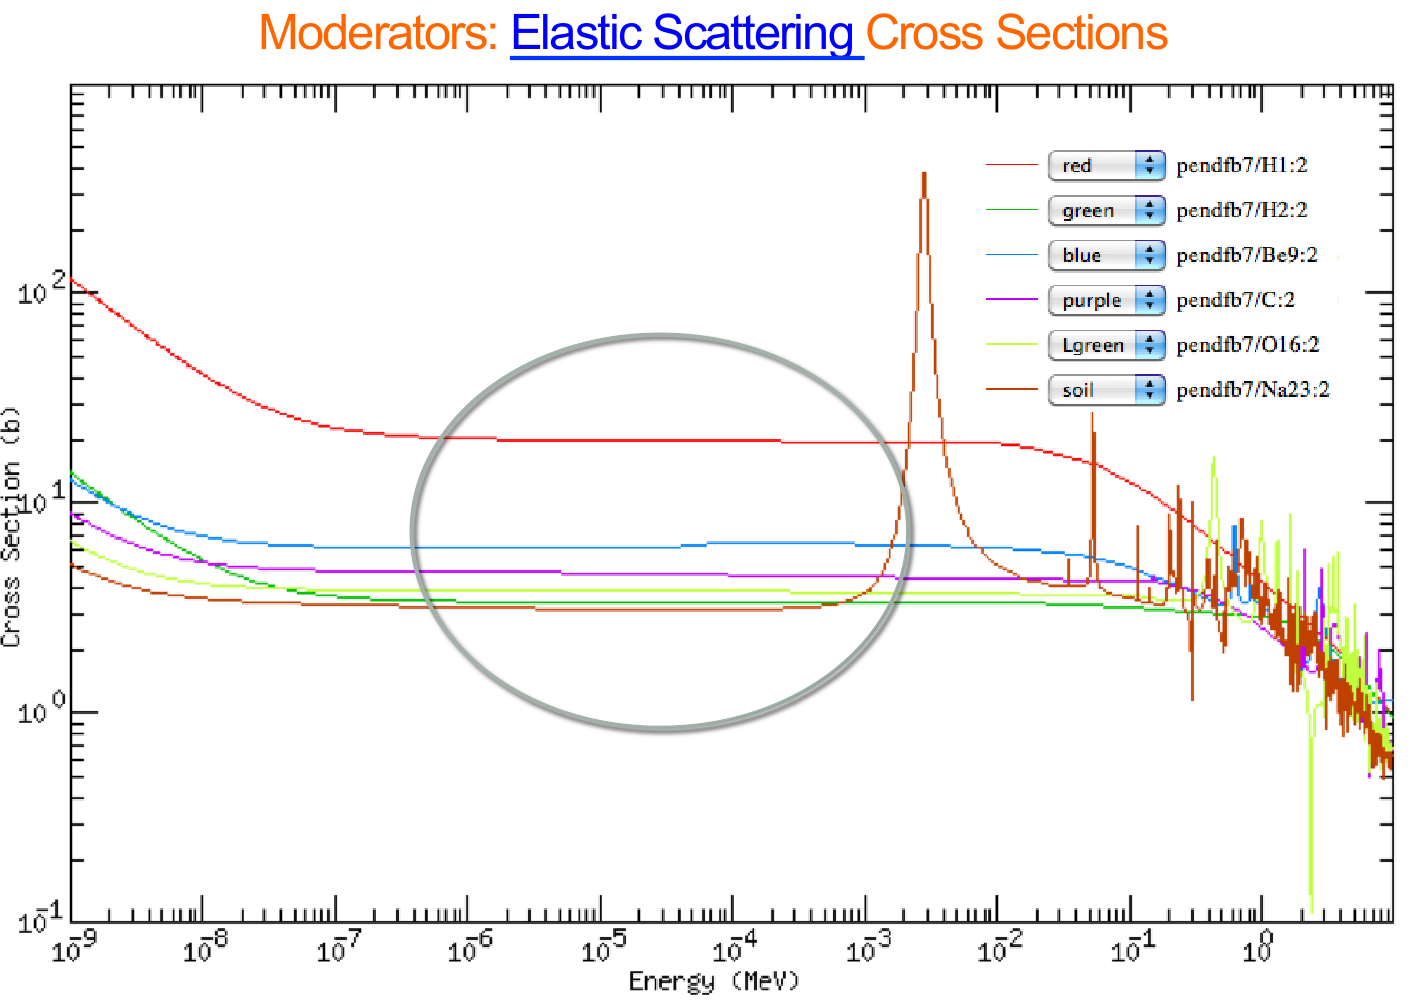
\includegraphics[width=6in]{images/intro/scatter-xs-moderator.png}
  \\
  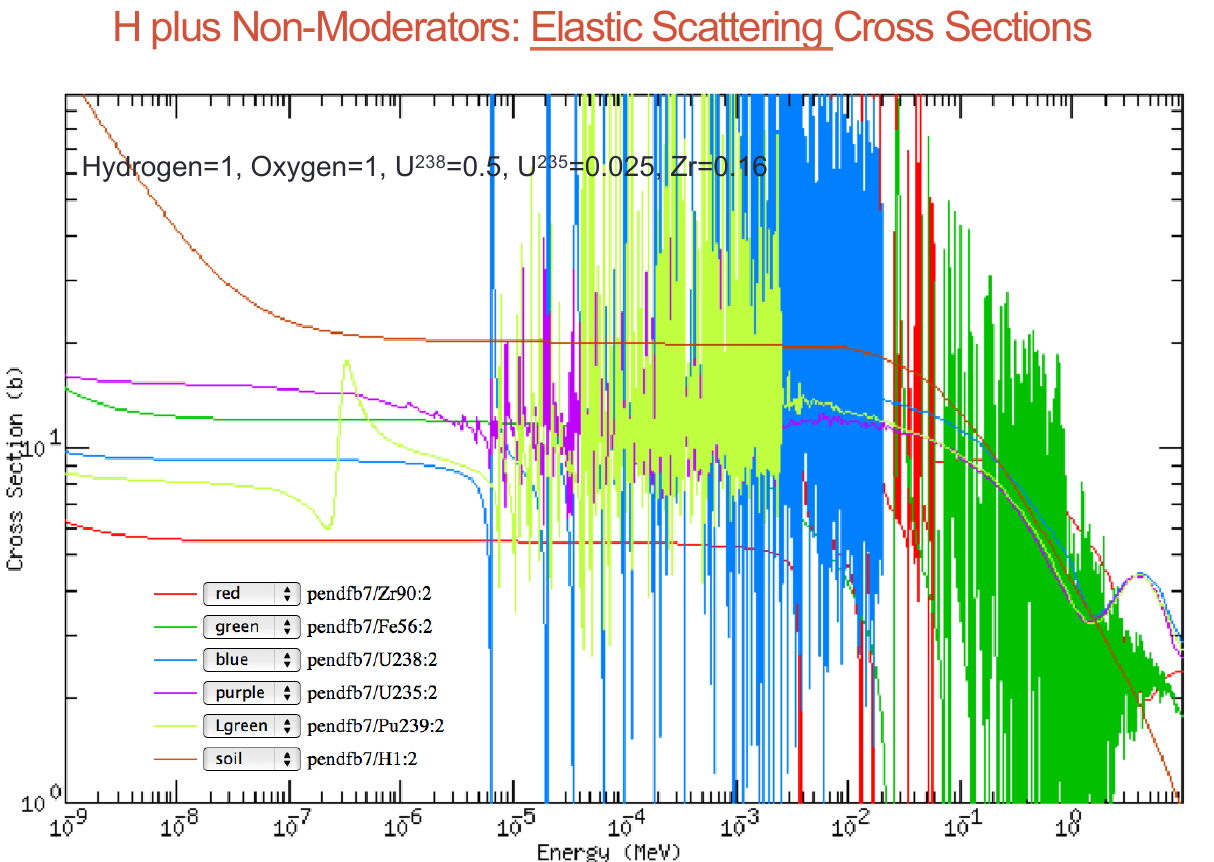
\includegraphics[width=6in]{images/intro/scatter-xs-LWR.png}
  \caption{Elastic Scattering Cross Sections} \label{scatter-xs}
\end{figure}

\item Capture cross section as in Figure~\ref{capture-xs}: 
  \begin{figure}
    \centering
    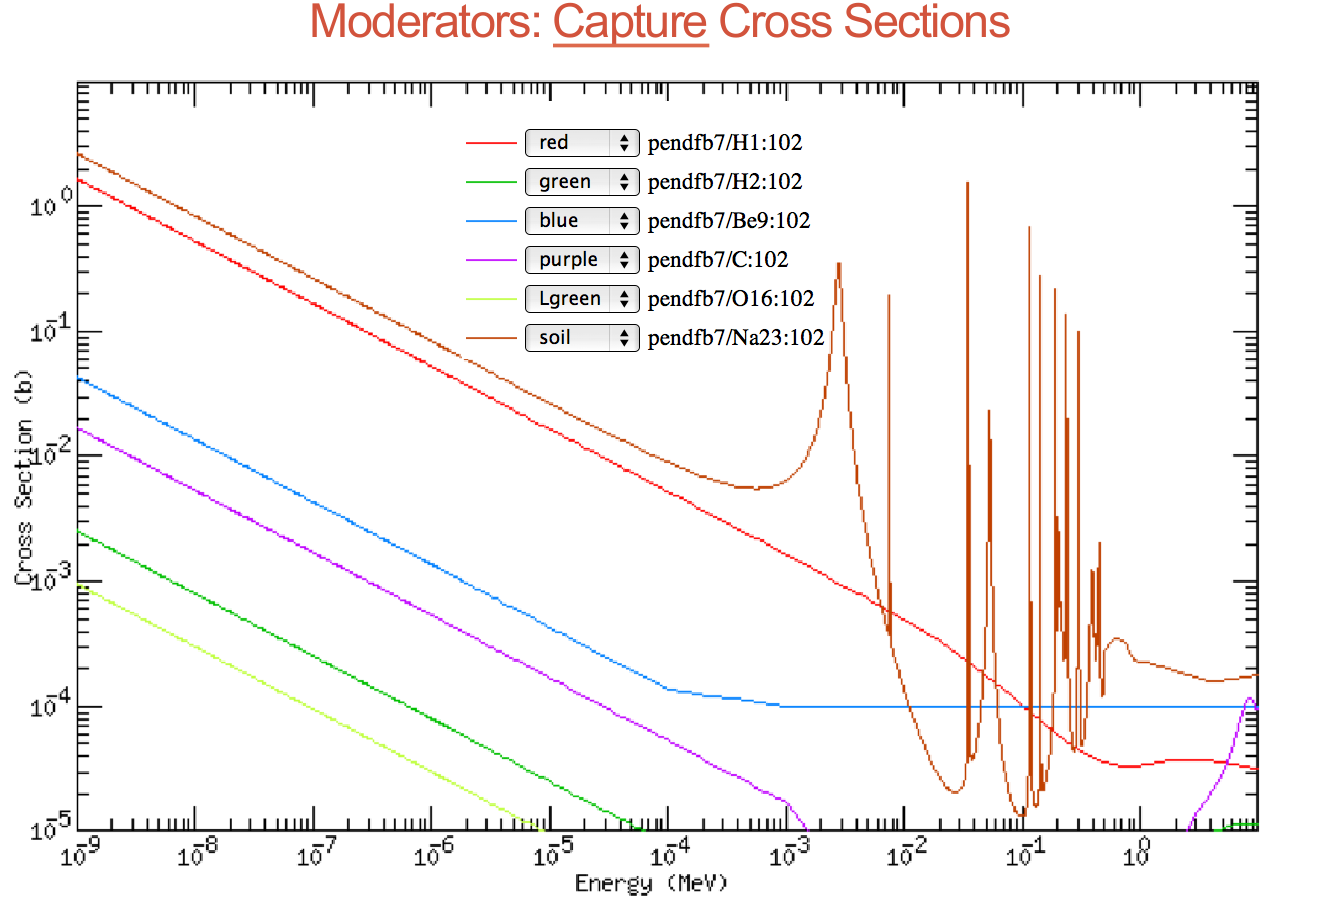
\includegraphics[width=6in]{images/intro/capture-xs.png}
    \\
    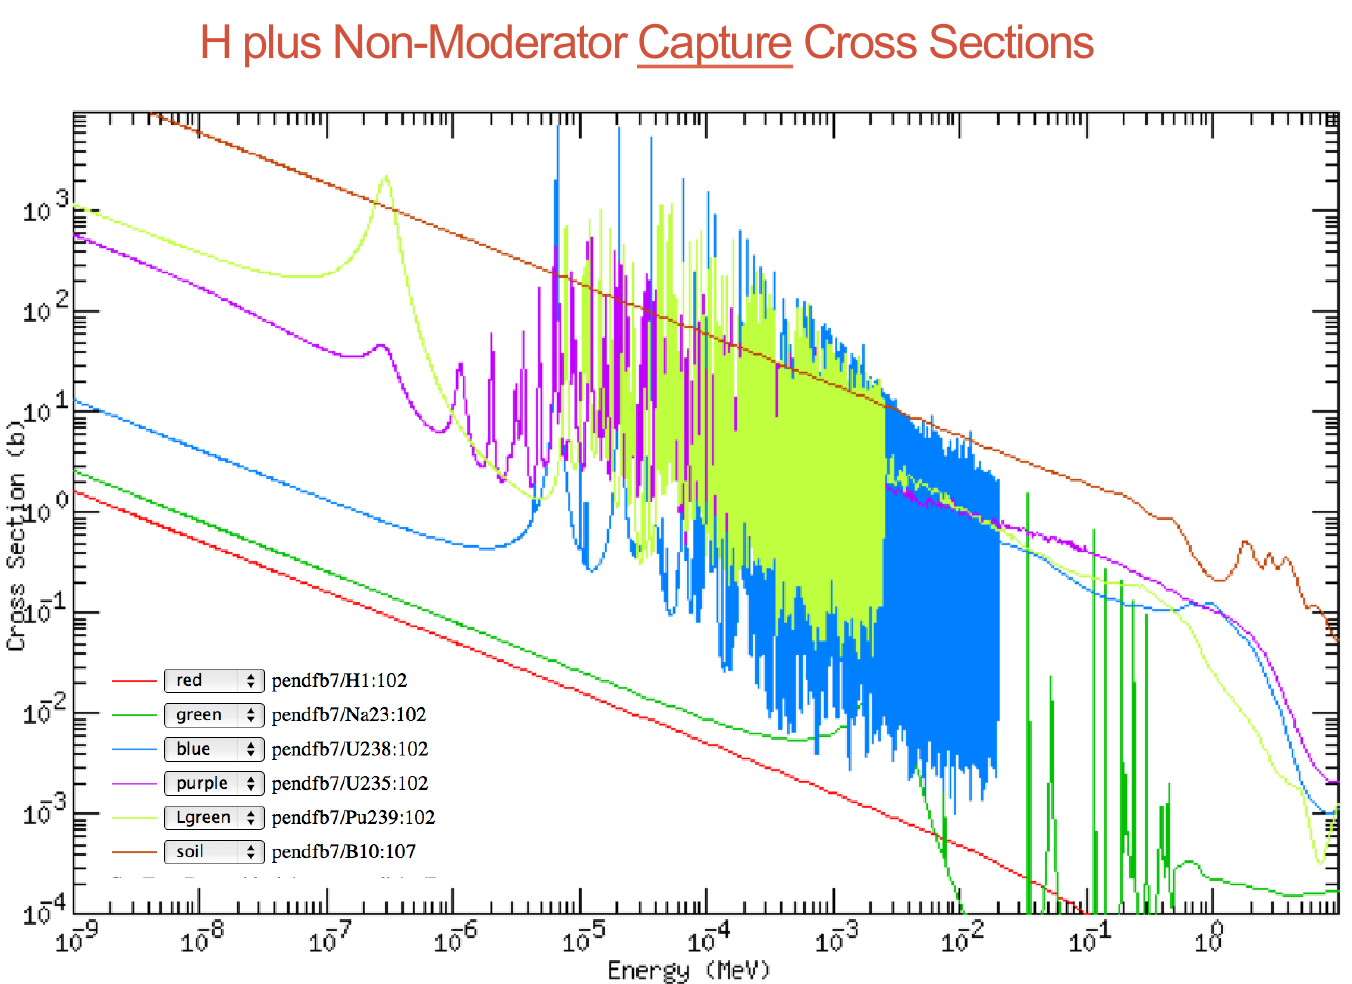
\includegraphics[width=6in]{images/intro/capture-xs-2.png}
    \caption{Capture Cross Section} \label{capture-xs}
  \end{figure}
  \begin{enumerate}
  \item H has no resonance; it has the highest scattering xs in LWR, so we can ignore any other isotopic's neutron scattering.   
  \item Na has a huge resonance in 23 keV, and more resonances at higher energies because it is a heavy isotope.
  \item Near zero energy,
    \eqn{ \sigma(E\to 0) \propto \sqrt{\frac{kT}{AE}}    }
  \item Resonance at 6 to 7 eV: U238. 
  \item U235's thermal elastic xs is larger than 238's, and they both have resonance around the same range.   
  \item A small resonance at .3 eV: Pu239 (its signiture is a super low energy scattering xs). 
  \end{enumerate}

\item Given an unknown material type, all we care is to count the nucleus density of each material and look at it's xs. 
\end{enumerate}


\clearpage
\topic{Steady State} 
\begin{enumerate}
\item A PWR typically have a Doppler coefficient of -3 pcm/K. 

\item One Group $\kinf$: in one group $k_{\infty}$ only depends on cross sections $k_{\infty} = \frac{\nu \Sigma_f}{\Sigma_a}$ and has no flux dependency. The flux is buried in the calculation of cross section.

\item Two group $\kinf$: we start with neutron balance equation:
  \begin{align}
    \frac{\nu \Sigma_{f1}}{k_{\infty}} \Phi_1 - \Sigma_{a1} \Phi_1 - \Sigma_{s12} \Phi_1 + \frac{\nu \Sigma_{f2}}{k_{\infty}} \Phi_2 + \Sigma_{s21} \Phi_2 &= 0 \\
\Sigma_{s12} \Phi_1 - \Sigma_{s21} \Phi_2 - \Sigma_{a2} \Phi_2 &= 0 
  \end{align}
  Typically what we do is to write it in a matrix form and solve for a coupled system. But even better, we can define the \hi{effective removal rate} $\bar{\Sigma}_{s12}$, and re-write the two-group balance equation: 
  \begin{align}
    \frac{\nu \Sigma_{f1}}{k_{\infty}} \Phi_1 - \Sigma_{a1} \Phi_1 - \bar{\Sigma}_{s12} \Phi_1 + \frac{\nu \Sigma_{f2}}{k_{\infty}} \Phi_2 &= 0 \\
    \bar{\Sigma}_{s12} \Phi_1- \Sigma_{a2} \Phi_2 &= 0 
  \end{align}
  Then we can solve for $\frac{\Phi_1}{\Phi_2}$ from the second equation in terms of cross section, plug in the first equation, and get $k_{\infty}$ from there. Notice that we only know the relative magnitude of $\Phi$ and $\Phi_2$. 

\item Know Two-group diffusion model: group 1 is the fast group larger than 0.625 eV, and group 2 is the thermal group. 
\begin{enumerate}
\item $D_1 = 1.5, D_2 = 0.5$.
\item Total fission source: $\chi_1 = 1.0, \chi_2 = 0.0$ implies that the fission source in thermal group is zero,
  \eqn{ S_f(\vecr) = \chi_g \Sum_g \nu \Sigma_{fg} (\vecr) \phi_g(\vecr) }
\item Scattering source: define effective down-scatter, so up-scattering is zero $\Sigma_{s21} (\vecr) = 0$. 
\item Final Two-Group Diffusion Equations: 
  \eqn{\boxed{ -\divergence D_1 \gradient \phi_1 + [\Sigma_{a1} + \Sigma_{s12} ] \phi_1 = \nu \Sigma_{f1} \phi_1 + \nu \Sigma_{f2} \phi_2 + S_1} }
  \eqn{\boxed{ -\divergence D_2 \gradient \phi_2 + \Sigma_{a2} \phi_2 = \Sigma_{s12} \phi_1 + S_2} }
\end{enumerate}

\item Know the one-group fundamental mode eigenvalues and eigenvectors as in Table~\ref{eigen-values}. 
\begin{table}[ht]
  \centering
  \begin{tabular}{|l|l|l|} \hline
     Slab $\in  \left[- \frac{L}{2}, \frac{L}{2} \right]$ & $\phi(x) = A \cos \left( \frac{\pi x}{L} \right)$ & $B^2 = \left( \frac{\pi}{L} \right)^2$ \\ \hline
     Sphere $\in [0, R]$ & $\phi(r)= A\frac{\sin \left( \frac{\pi r}{R} \right)}{r} $ & $B^2 = \left( \frac{\pi}{R} \right)^2$ \\ \hline
     Infinite cylinder $\in [0, R]$ & $\phi(r) = A J_0 \left( \frac{2.405 r}{R} \right)$ & $B^2 = \left( \frac{2.405}{R} \right)^2$ \\ \hline
     Finite cylinder $r \in [0, R], z \in \left[ -\frac{H}{2}, \frac{H}{2} \right]$ & $\phi(r,z) = A J_0\left( \frac{2.405 r}{R} \right) \cos \left( \frac{\pi z}{H} \right)$ & $B^2 = \left( \frac{2.405}{R} \right)^2 + \left( \frac{\pi}{H} \right)^2$ \\ \hline
     Parallelepiped $\in \left[ -\frac{L_i}{2}, \frac{L_i}{2} \right]$ & $\phi(x) = A \cos \left( \frac{\pi x}{L_x} \right) \cos \left( \frac{\pi y}{L_y} \right) \cos \left( \frac{\pi x}{L_z} \right)$ & $B^2 = \left( \frac{\pi}{L_x} \right)^2 + \left( \frac{\pi}{L_y} \right)^2 + \left( \frac{\pi}{L_z} \right)^2$ \\ \hline
  \end{tabular}
\end{table}

\end{enumerate}




\clearpage
\topic{Kinetics}








\end{document}
